\chapter{Robustly disjoint sr-paths}

We say that two sr-paths $p_1$ and $p_2$ are \emph{robustly disjoint} with respect to $\fset$ if and only if $p_1, p_2$ are disjoint and 

$$
\forall f \in F \ \forall s \subseteq f \quad forw(p, s) \cap forw(p, f \setminus s) = \emptyset
$$


\begin{lemma}
\label{lemma:edgesoutforw1}
Let $p$ be a sr-path and $f \subseteq E(G)$. Then
$$
\forw(p, f) = \forw(p, f \cap \forw(p))
$$
\end{lemma}

\begin{proof}
\todo~Inuititon: removing an edge that is not used by $p$ cannot affect it.
\end{proof}

\begin{corollary}
\label{cor:edgesoutforw2}
Let $p$ be a sr-path and $s \subseteq f \subseteq E(G)$. If $s \cap \forw(p) = \emptyset$ then $\forw(p, f) = \forw(p, f \setminus s)$.
\end{corollary}

\begin{proof}
Since $s \cap \forw(p) = \emptyset$, we have that $f \cap \forw(p) = (f \setminus s) \cap \forw(p)$.
Hence, by Lemma \ref{lemma:edgesoutforw1} it holds that
$$
\forw(p, f) = \forw \left(p, f \cap \forw(p) \right) = \forw \left(p, (f \setminus s) \cap \forw(p)\right) = \forw(p, f \setminus s).
$$
\end{proof}

\begin{theorem}
If two sr-paths $p_1, p_2$ are robustly disjoint with respect to $\fset$ then,
for all $f \in F$, $p_1$ and $p_2$ are disjoint on $G \setminus f$.
\end{theorem}

\begin{proof}
Suppose that there exists $f \in F$ such that $p_1$ and $p_2$ are not disjoint on $G \setminus f$.
In other words, $\forw(p_1, f) \cap \forw(p_2, f) \neq \emptyset$. Let $e$ be an edge belonging to
this intersection. Let $s = f \cap \forw(p_1)$. By Lemma \ref{lemma:edgesoutforw1} we have that
$$
\forw(p_1, f) = \forw(p_1, s).
$$

Since $p_1, p_2$ are disjoint, we have $\forw(p_1) \cap \forw(p_2) = \emptyset$. Thus, since $s \subseteq \forw(p_1)$,
it holds that $s \cap \forw(p_2) = \emptyset$. Therefore, by Corollary \ref{cor:edgesoutforw2},

$$
\forw(p_2, f) = \forw(p_2, f \setminus s).
$$

This is a contradition. Since $p_1$ and $p_2$ are robustly disjoint, in particular
$\forw(p_1, s) \cap \forw(p_2, f \setminus s) = \emptyset$, and hence

$$
e \in \forw(p_1, f) \cap \forw(p_2, f) = \forw(p_1, s) \cap \forw(p_2, f \setminus s) = \emptyset.
$$

\note{to make the algorithms more efficient we could define a relaxed version of robustness. if we enfore that
for each $f$ in $F$ either $f \cap \forw(p_1) = \emptyset$ or $f \cap \forw(p_2) = \emptyset$ then the old algorithm works.
this means that less pairs of robustly disjoint paths exists but whenever we find one then it will be robust.}
\end{proof}

\section{Better definition}


We say that two sr-paths $p_1$ and $p_2$ are \emph{robustly disjoint} with respect to $\fset$ if and only if $p_1, p_2$ are disjoint and 
for all $f \in F$, $p_1$ and $p_2$ are disjoint on $G \setminus f$, that is, $\forw(p_1, f) \cap \forw(p_2, f) = \emptyset$. 

\begin{lemma}
Let $p = \langle x_1, \ldots, x_k \rangle$ and $F \subseteq \powerset(E)$. Then
$$
\forw(p, f) = \bigcup_{i = 2}^k \forw(x_{i - 1}, x_i, f).
$$
\end{lemma}

\begin{proof}
Let $e \in \forw(p, f)$. Then $e \in \forw(p)$ on $G \setminus f$. This means that there exists $i \in \{2, \ldots, k\}$ such that
$e$ belongs to a shortest path from $x_{i - 1}$ to $x_i$ on $G \setminus f$. Thus $e \in \forw(x_{i - 1}, x_i, f)$.

On the other hand, if $e \in \bigcup_{i = 2}^k \forw(x_{i - 1}, x_i, f)$ then there exists $i$ such that $e \in \forw(x_{i - 1}, x_i, f)$.
Hence $e$ belongs to a shortest path from $x_{i - 1}$ to $x_i$ on $G \setminus f$. Hence $e \in \forw(p, f)$.
\end{proof}

\begin{theorem}
Two sr-paths $p_1 = \langle x_1, \ldots x_k \rangle$ and $p_2 = \langle y_1, \ldots, y_r \rangle$ are robustly disjoint if and only if
for all $i = 2, \ldots, k$ and $j = 2, \ldots, r$, $\langle x_{i - 1}, x_i \rangle$ and $\langle y_{j - 1}, y_j \rangle$ are robustly disjoint.
\end{theorem}

\begin{proof}
$(\Rightarrow)$ Suppose that $p_1, p_2$ are robustly disjoint and that there exists $i$ and $j$ such that $\langle x_{i - 1}, x_i \rangle$ and
$\langle y_{j - 1}, y_j \rangle$ are not robustly disjoint. Then there exists $f \in F$ such that 
$\forw(x_{i - 1}, x_i, f) \cap \forw(y_{j - 1}, y_j, f) \neq \emptyset$.
Thus,
\begin{align*}
\forw(x_{i - 1}, x_i, f) \cap \forw(y_{j - 1}, y_j, f) & \subseteq 
\left( \bigcup_{i = 2}^k \forw(x_{i - 1}, x_i, f) \right) \cap \left( \bigcup_{j = 2}^r \forw(y_{j - 1}, y_j, f) \right) \\
& = \forw(p_1, f) \cap \forw(p_2, f) 
\end{align*}
contradicting the fact that $p_1, p_2$ are robustly disjoint.

$(\Leftarrow)$ Suppose that for all $i = 2, \ldots, k$ and $j = 2, \ldots, r$,  $\langle x_{i - 1}, x_i \rangle$ and $\langle y_{j - 1}, y_j \rangle$
are robustly disjoint and that $p_1, p_2$ are not. Then there exists $f \in F$ such that $\forw(p_1, f) \cap \forw(p_2, f) \neq \emptyset$. Since 
$\forw(p_1, f) = \bigcup_{i = 2}^k \forw(x_{i - 1}, x_i, f)$ and $\forw(p_2, f) = \bigcup_{j = 2}^r \forw(y_{j - 1}, y_j, f)$ there exists $i$ and $j$
such that 
$$
\forw(x_{i - 1}, x_i, f) \cap \forw(y_{j - 1}, y_j, f) \neq \emptyset
$$ 
contradicting our assumption.
\end{proof}

\section{Other stuff}

We have seen in the experimental results that the practical robustness of rodubslty disjoint paths for single link failures
is ofter much larger. In many cases, disjointness is preserved for larger sets of failures. This lead us to think about whether
or not we can compute the effective robustness of a given pair of sr-paths.

\begin{problem}{Effective robustness}
\label{prob:eff-rob}
Given a network $G$ and two sr-paths $p_1, p_2$, what is the minimum size of an edge set $F \subseteq E(G)$
so that $p_1$ and $p_2$ are not disjoint on $G \setminus F$.
\end{problem}

\begin{theorem}
Problem \ref{prob:eff-rob} is \NPhard. 
\end{theorem}

\begin{proof}
\todo{
To prove that this problem is \NPhard, we are going to reduce to the following problem:
what is the minimum number of edges that we need to delete to make the shortest path
from $s$ to $t$ cost at least $d$? Make sure that \cite{Golovach2011PathsOB}
has the problem that we want.

\begin{center}
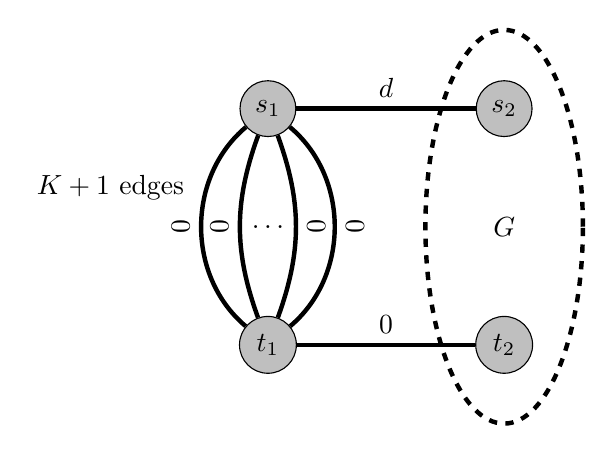
\begin{tikzpicture}
\node[draw, circle, fill=lightgray] (s1) at (0, 0) {$s_1$};
\node[draw, circle, fill=lightgray] (s2) at (3, 0) {$s_2$};
\node[draw, circle, fill=lightgray] (t1) at (0, -3) {$t_1$};
\node[draw, circle, fill=lightgray] (t2) at (3, -3) {$t_2$};

\draw (s1) edge[ultra thick, bend left = 50, sloped, above] node {$0$} (t1);
\draw (s1) edge[ultra thick, bend left = 20, sloped, above] node {$0$} (t1);
\draw (s1) edge[ultra thick, bend right = 50, sloped, above] node {$0$} (t1);
\draw (s1) edge[ultra thick, bend right = 20, sloped, above] node {$0$} (t1);

\node at (0, -1.5) {$\ldots$};

\node at (-2, -1) {$K + 1$ edges};


\draw (s1) edge[ultra thick, above] node {$d$} (s2);
\draw (t1) edge[ultra thick, above] node {$0$} (t2);

\draw[ultra thick, dashed] (3, -1.5) ellipse (1 and 2.5);

\node at (3, -1.5) {$G$};

\end{tikzpicture}
\end{center}

$G$ is the input graph for the shortest path edge deletion problem. 
$K$ is the minium $s_2$, $t_2$ cut in $G$. We can assume that the shortest path
from $s_2$ to $t_2$ is less than $d$ otherwise the problem is trivial.
The shortest path form $s_1$ to $t_1$ will always be one of the $0$ cost edges
since there are $K + 1$ edges. The answer to our problem is the minimum number of edges
such that the shortest path from $s_2$ to $t_2$ becomes $(s_2, s_1, t_1, t_2)$. This
happens iff we remove edges from $G$ making the shortest path from $s_2$ to $t_2$
cost more than $d$.
}

\end{proof}

